\documentclass[]{beamer}
%\usepackage[MeX]{polski}
%\usepackage[cp1250]{inputenc}
\usepackage{polski}
\usepackage[utf8]{inputenc}
\beamersetaveragebackground{green!12}
\usetheme{Copenhagen}
\usecolortheme[rgb={0.2,0.5,0.2}]{structure}
\usepackage{beamerthemesplit}
\usepackage{multirow}
\usepackage{multicol}
\usepackage{array}
\usepackage{graphicx}
\usepackage{enumerate}
\usepackage{amsmath} %pakiet matematyczny
\usepackage{amssymb} %pakiet dodatkowych symboli
\author{Patryk Wojciekian}
\title{Archer}
\subtitle{Niszczyciel czołgów}
\date{}

\begin{document}

\begin{frame}
\maketitle
\end{frame}

\begin{frame}
\frametitle{Krótkie przedstawienie}
\begin{figure}[here]
\begin{center}
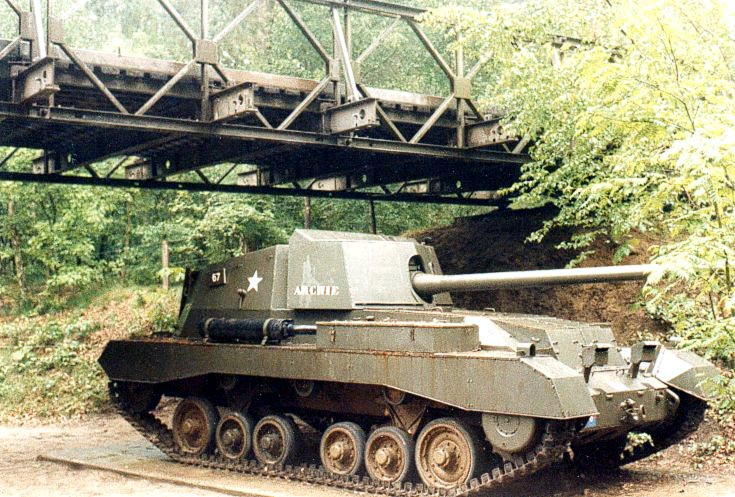
\includegraphics[scale=0.8]{Archer.jpg}
\end{center}
\end{figure}
Archer (ang. ,,Łucznik'') - brytyjski niszczyciel czołgów (przeciwpancerne działo samobieżne) z okresu II wojny światowej.
\end{frame}

\begin{frame}
\frametitle{Wyposażenie}
Archer został wyposażony w armatę 17-funtową (76,2mm), a także ręczny karabin maszynowy Bren kalibru 7,7mm.

\par \ 
\begin{columns}
\column{0.3\textwidth}
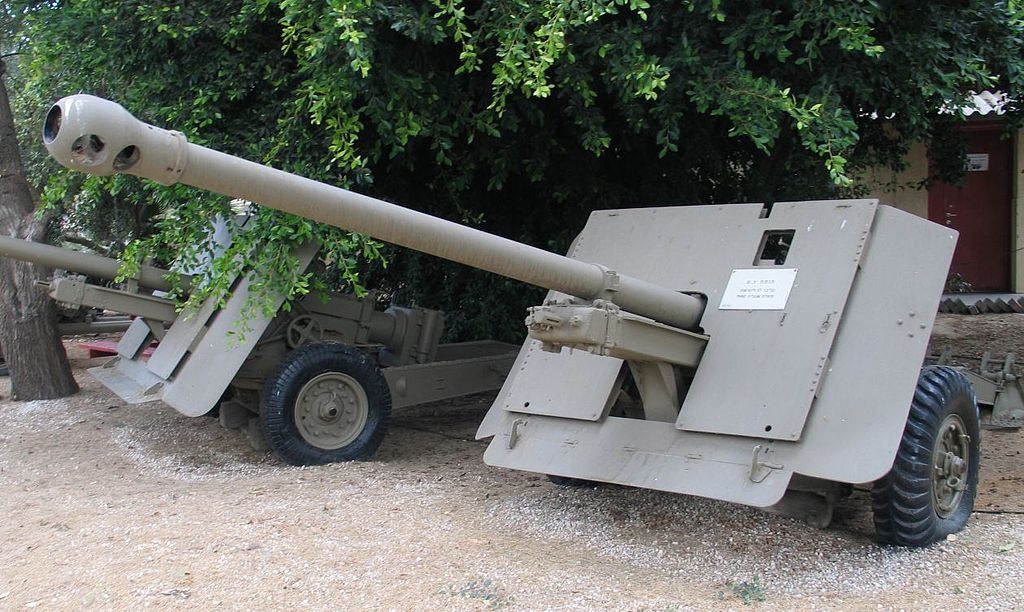
\includegraphics[scale=0.3]{dzialo.jpg}
\column{0.3\textwidth}
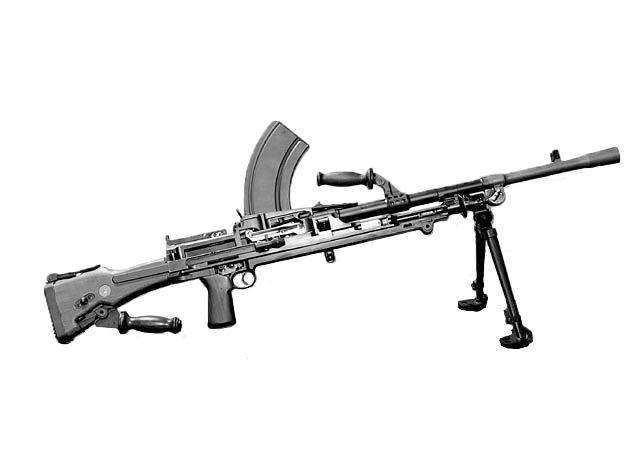
\includegraphics[scale=1.31]{Bren.jpg}
\end{columns}
\end{frame}

\begin{frame}
\frametitle{Czym się wyróżniał?}
Archer miał prostą, ale i niekonwencjonalną konstrukcję. Cienki pancerz (10-20mm) był jego piętą Achillesową, aczkolwiek jego działo miało dostatecznie wielką siłę, aby móc niszczyć najcięższe niemieckie czołgi.
\end{frame}
\begin{frame}
\frametitle{Produkcja}
Ich produkcja rozpoczęła się w marcu 1944, jednak szybko się zatrzymała \pause - gdyż już na początku 1945 roku wstrzymano dalszą produkcję. \pause

Ostatecznie wyprodukowano 655 czołgów typu ,,Archer''.
\end{frame}

\begin{frame}
\frametitle{Praktyczność na froncie}
Pojazd był idealny do atakowania z zasadzki, gdyż jego niska sylwetka umożliwiała łatwe jego ukrycie, a dzięki temu, że przód pojazdu był skierowany w przeciwną stronę od przeciwnika, można było łatwiej opuścić stanowisko bojowe.

Niestety utrudniał ten manewr fakt, że kierowca musiał opuszczać swoje stanowisko, gdyż w to miejsce cofał się zamek armaty.
\end{frame}

\begin{frame}
\frametitle[toc=]{Praktyczność na froncie cd.}
Nie był to jednak sprzęt lubiany przez załogi. Krytykowano go za zbyt cienki pancerz, a także niewygodę obsługi. Chętnie udostępniano je więc sojusznikom. Takim sposobem kilka czołgów typu ,,Archer'' trafiło na uzbrojenie polskich armii.
\end{frame}

\begin{frame}
\frametitle{Użyteczność po wojnie}
Ze względu na dużą skuteczność armaty pozostawały w uzbrojeniu do początku lat 50. \pause 

Po tym czasie pojazdy zostały wycofane z jednostek brytyjskich. Zakupił je Egipt i użył ich w wojnie z koalicją brytyjsko-francusko-izraelską w czerwcu 1956. \pause

Po walce, z 44 Archerów zostały 4 sztuki, reszta została zniszczona.
\end{frame}

\begin{frame}
\frametitle{Źródła}
pl.wikipedia.org/wiki/Archer\_(niszczyciel\_czo\%C5\%82g\%C3\%B3w)
\end{frame}
\begin{frame}
\begin{center}
Dziękuję za uwagę.
\end{center}
\end{frame}
\end{document}
